\documentclass[12pt]{article}
\usepackage{tikz}
\usepackage{amssymb}
\usepackage{amsmath}
\usepackage{breqn}

\usetikzlibrary{automata, positioning, arrows}

\title{SE 3310 Theoretical Foundations of Software Engineering Assignment 2}
\author{Marcus Tuen Muk}
\date{February 09 2023}


\begin{document}

    \begin{titlepage}
        \clearpage\maketitle
        \thispagestyle{empty}
    \end{titlepage}

    \section{Regular Expressions}
        \subsection{\[L_a = \{wwwa^n:w \in \{a,b\}, n > 0\}\]}
            \indent
            Based on this language, w is either all a or all b. This language is a regular language.
            \begin{figure}[ht]
                \centering
                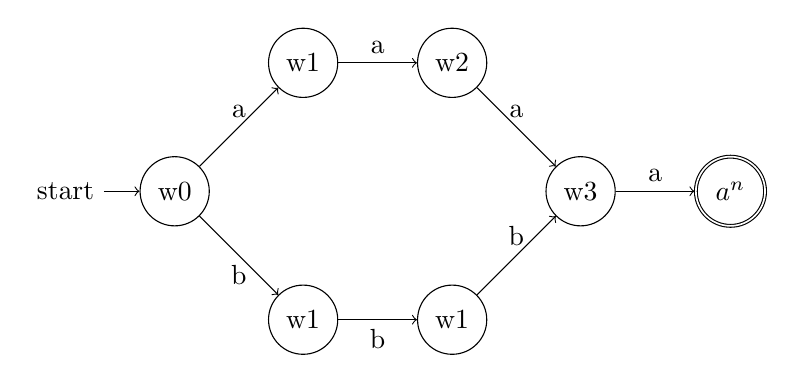
\begin{tikzpicture}
                    \node[state, initial] (w0) {w0};
                    \node[state, above right = of w0] (a1) {w1};
                    \node[state, right = of a1] (a2) {w2};
                    \node[state, below right =of w0] (b1) {w1};
                    \node[state, right =of b1] (b2) {w1};
                    \node[state, below right =of a2] (w3) {w3};
                    \node[state, accepting, right =of w3] (an) {\(a^n\)};
                    

                    \draw   (w0) edge[->, right, above] node{a} (a1)
                            (w0) edge[->, right, below] node{b} (b1)
                            (a1) edge[->, right] node[above] {a} (a2)
                            (b1) edge[->, right] node[below] {b} (b2)
                            (a2) edge[->, right] node[above] {a} (w3)
                            (b2) edge[->, right] node[above] {b} (w3)
                            (w3) edge[->, right] node[above] {a} (an);
                        
                \end{tikzpicture}  
            \end{figure}
        
                
\end{document}